% IEEE conference-paper CANDIDATE - Chennai urban flood-risk project (B794)
% Status: draft for author and supervisor review. Author names/affiliations are placeholders on purpose.
\documentclass[conference]{IEEEtran}
\usepackage{graphicx}
\usepackage{booktabs}
\usepackage{amsmath}
\usepackage{url}
\usepackage{siunitx}
\usepackage[hidelinks]{hyperref}
\graphicspath{{figures/}}

\begin{document}

\title{What Reported Floods Can and Cannot Teach: An Evidence-Aware Multi-Source Framework for Urban Flood Assessment in Chennai, India}

\author{\IEEEauthorblockN{[Author 1]\quad [Author 2]}
\IEEEauthorblockA{[Department], [Institution], [City], India\\ \relax
\mbox{[email addresses]}}
\and
\IEEEauthorblockN{[Supervisor]}
\IEEEauthorblockA{[Department], [Institution]}}

\maketitle

\begin{abstract}
Urban flood studies in data-scarce cities often train classifiers on whatever flood records exist, then report accuracy. We present a reproducible framework for Chennai, India, that combines relative terrain susceptibility (30\,m, seven DEM-derived indicators), Sentinel-1 backscatter diagnostics for eight 2021 acquisitions, exposure and partial vulnerability indicators, and administrative and crowd-sourced flood reports. Every input carries an explicit evidence class. The only independent flood references obtainable were reported locations: 561 (2021) and 306 (2015) inundated locations listed by the Greater Chennai Corporation, and 2{,}350 crowd-flagged street segments (2 December 2015; 2{,}307 inside the region). They give the monsoon year only. We re-verified the published depth classes against the source document and found column-shift errors in a public extraction. The two independent 2015 sources agree spatially 2.5 times more often than a street-network null model. 2021 reports show no association with bright-backscatter radar components at 0--100\,m. Treating reported wards as presences and all other wards as unlabelled, we evaluated whether any indicator set ranks reported wards above the background, using zone-blocked, buffered cross-validation and label-permutation nulls. None of 12 indicator--model combinations exceeds its null (permutation $p \ge 0.24$); the only nominally significant model is a ward-area-only control (2021). Reporting-based labels in this setting encode reporting opportunity rather than a learnable physical signal. We therefore release exploratory structure (two stable ward clusters, Moran's $I$ up to 0.77) and a data contract specifying what supervised flood prediction would require, instead of a prediction map.
\end{abstract}

\begin{IEEEkeywords}
urban flooding, Sentinel-1, flood susceptibility, presence-background analysis, spatial cross-validation, exposure, vulnerability, Chennai
\end{IEEEkeywords}

\section{Introduction}
Chennai has flooded repeatedly, most severely in November--December 2015 and again during the 2021 northeast monsoon. Satellite and modelling studies of the 2015 event map large inundated areas \cite{ramasamy2018chennai,chundeli2018chennai,iwmi2015chennai}. Machine-learning studies often build flood ``susceptibility'' or ``prediction'' maps from such inventories. When the labels are uncertain, temporally coarse or produced by the same sensor used as a predictor, the resulting accuracy figures can describe the labels more than the floods.

This paper asks a narrower question: \emph{given the flood evidence that can actually be obtained and verified for Chennai, what can a multi-source geospatial framework legitimately establish?} We contribute:
\begin{enumerate}
\item an integrated, reproducible pipeline that keeps susceptibility, exposure, vulnerability and flood evidence as separate, hash-verified layers with explicit evidence classes (E1 mapped extent to E5 context);
\item a source-level verification of an official ward-level inundation list, including correction of a published extraction;
\item a presence-background evaluation with spatial blocks, buffers, permutation nulls and an area control, showing that the available labels do not support a learned flood model;
\item an open dashboard and data contract that carry these limits into use.
\end{enumerate}

\section{Related Work}
Terrain indices such as the topographic wetness index (TWI) \cite{beven1979twi} and height above nearest drainage (HAND) \cite{nobre2011hand} are standard building blocks of susceptibility models. Sentinel-1 C-band SAR \cite{torres2012s1} is widely used for flood mapping. In cities, however, open water appears dark only where it is visible to the radar. Flooded streets can instead brighten through double bounce, and layover and shadow hide much of the ground \cite{mason2018urban,chini2019coherence,zhao2024review}. Risk frameworks separate hazard, exposure and vulnerability \cite{ipcc2012srex}. Composite social vulnerability indices \cite{cutter2003sovi} require demographic inputs that are often unavailable at ward level in Indian cities. Presence-only data are routine in species-distribution modelling, where presence-background discrimination \cite{phillips2006maxent} and positive-unlabelled learning \cite{elkan2008pu} replace accuracy against true negatives. Spatially structured data require blocked cross-validation \cite{roberts2017cv,valavi2019blockcv}. We carry these practices into urban flood assessment.

\section{Study Area and Data}
The analysis grid is EPSG:32644 at 30\,m ($1416\times726$ cells). It covers a provisional, OpenStreetMap-derived study area of about 435\,km$^2$ (483{,}727 cells), which is \emph{not} the official corporation boundary. Analysis units are the 200 wards of the Greater Chennai Corporation (GCC) from the state GIS (TNGIS, 432\,km$^2$). Table~\ref{tab:data} summarises the inputs and their evidence classes. Rainfall from CHIRPS \cite{funk2015chirps} is context only: about 29 native 0.05$^\circ$ cells intersect the study area. Sentinel-1A IW GRD scenes (descending, relative orbit 92, about 06:01 IST) were processed in Google Earth Engine \cite{gorelick2017gee} for eight dates between 5 September and 28 November 2021.

\begin{table}[t]
\caption{Inputs, roles and evidence classes}
\label{tab:data}
\centering\footnotesize
\begin{tabular}{@{}p{2.6cm}p{3.3cm}c@{}}
\toprule
Input & Role & Class \\
\midrule
GLO-30 DSM (30\,m) & terrain indicators, SUS-1 & -- \\
Sentinel-1 VV/VH, 8 dates & dark candidates, bright-VV diagnostics & E4 \\
GCC CDMP 2026 lists \cite{gcc2026cdmp} & inundated locations, 2015 and 2021 & E3 \\
Crowd-flagged streets & 2,350 segments, 2 Dec 2015 & E3 \\
CHIRPS v3, IMD & antecedent rainfall & E5 \\
CDMP ward tables; WorldPop 2020 \cite{tatem2017worldpop} & population (two sources) & -- \\
TNGIS roads, facilities & exposure & -- \\
Slum polygons; health; relief & partial vulnerability & -- \\
\midrule
Mapped flood extent & \emph{not obtained} & E1: none \\
\bottomrule
\end{tabular}
\end{table}

\section{Methods}
\subsection{Relative susceptibility (SUS-1)}
Seven indicators (elevation, slope, TWI, log flow accumulation, distance to drainage, a Euclidean HAND proxy, fill depth) are rank- or robust-min--max scored within the scored domain and averaged with equal weights. Water-signature and missing cells (12{,}255) are \emph{not assessed} and never scored as low. A six-indicator variant without TWI agrees closely (Spearman 0.982; top-decile Jaccard 0.890) and is kept as a sensitivity case only. The index is relative, uncalibrated and not a probability.

\subsection{Flood evidence and its verification}
The GCC City Disaster Management Plan prints, per ward, the locations inundated in each monsoon year with a depth class (${<}2$, 2--3, 3--5, ${>}5$\,ft). A public table extraction was re-read against the PDF: for every page, the rotated column headers were recovered from the character stream and each printed mark was assigned to its nearest header, row by row. This verified 1{,}312 of 1{,}401 rows and exposed column shifts in the extraction: the 3--5\,ft class was lost in 72 rows and relabelled in 78 more. Locations were placed by a gazetteer within their printed ward. Each received a positional uncertainty of 50--750\,m by match type, and unplaced records were kept, not dropped. The project's reference checker classified the 2021 list as \textsc{presence\_only} and both 2015 sets as \textsc{qualitative\_only} with respect to the 2021 radar dates.

\subsection{Null-model comparisons}
For two sets of reports, or reports versus radar components, we report the share of locations within $d$ of the other set, divided by the same share for random points on the street network (representative points of 34{,}355 road polygons). We use 200 draws.

\subsection{Evidence-aware ward analytics}
For 198 wards with complete data, 14 indicators are log-transformed where skewed and standardised. They cover SUS-1, terrain, Sentinel-1, exposure and vulnerability. Report-derived quantities, coarse rainfall and partial-coverage population are excluded. We report:
\begin{enumerate}
\item principal components;
\item $k$-means clusters selected by silhouette \cite{rousseeuw1987silhouette} subject to bootstrap stability (adjusted Rand index \cite{hubert1985ari} $\ge 0.75$, 100 resamples);
\item Moran's $I$ \cite{moran1950} with contiguity weights;
\item a presence-background analysis.
\end{enumerate}
In the presence-background analysis, wards with $\geq 1$ listed location in an event year are presences. All others are \emph{background}, explicitly not negatives. Logistic regression and random forests \cite{breiman2001rf,pedregosa2011sklearn} are evaluated by out-of-fold presence-background AUC (PB-AUC) under leave-one-zone-out cross-validation (15 zones). Training wards within 500\,m of the test zone are removed. Each PB-AUC is compared with a label-permutation null that re-runs the full cross-validation (100 permutations for logistic regression, 20 for random forests). Controls are a ward-area-only model, a population-density-only model, and cross-event transfer (2015$\to$2021 and back).

\section{Results}
\subsection{Reported evidence}
The 2015 sources are mutually consistent (Fig.~\ref{fig:evidence}, Table~\ref{tab:cmp}). GCC locations lie within 50\,m of a crowd-flagged street 2.51 times as often as street-null points do (0 of 200 null draws reached the observed share). The reverse direction gives 2.27. In 2021, the GCC locations are no closer to bright-VV components than random street points at 0 and 100\,m (ratios 0.37--1.09). The only small excess occurs at 250\,m on two dates (97--98\% of reports vs.\ null means of 93--95\%). Ninety-six wards are listed in both years, but only seven exact location names recur.

\begin{table}[t]
\caption{Presence-only comparisons against a street-network null}
\label{tab:cmp}
\centering\footnotesize
\begin{tabular}{@{}lccc@{}}
\toprule
Comparison & $d$ (m) & Obs./null & Null$\ge$obs. \\
\midrule
CDMP 2015 $\to$ crowd streets 2015 & 50 & 2.51 & 0.00 \\
CDMP 2015 $\to$ crowd streets 2015 & 250 & 1.29 & 0.00 \\
Crowd streets $\to$ CDMP 2015 & 50 & 2.27 & 0.00 \\
CDMP 2021 $\to$ bright VV, 28 Nov & 100 & 1.03 & 0.27 \\
CDMP 2021 $\to$ bright VV, persistent & 0 & 0.37 & 0.99 \\
\bottomrule
\end{tabular}
\end{table}

\begin{figure}[t]
\centering
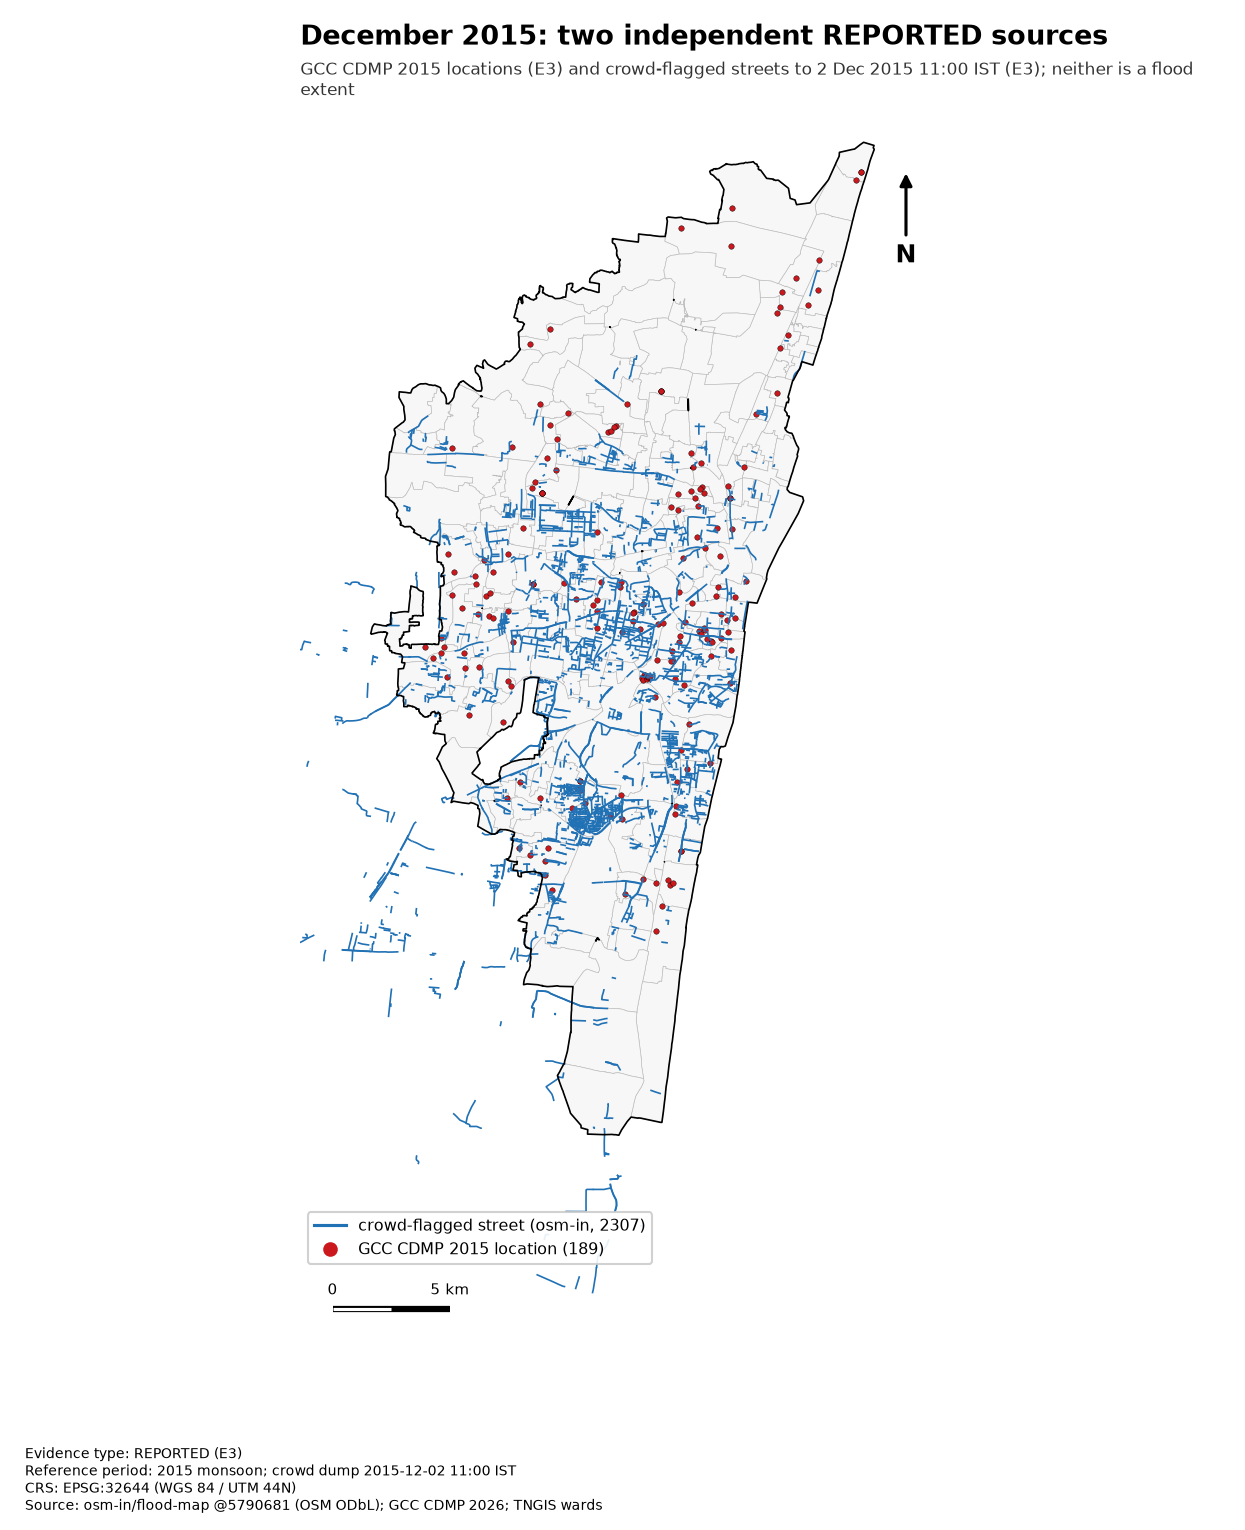
\includegraphics[width=0.85\columnwidth]{map_A2_2015_two_reported_sources.png}
\caption{Two independent reported sources for 2015: GCC CDMP locations (red) and crowd-flagged streets to 2 December 2015, 11:00 IST (blue). Neither is a flood extent.}
\label{fig:evidence}
\end{figure}

\subsection{Ward structure}
PC1 explains 46\% of the indicator variance. It contrasts low-lying, flat, drainage-proximal wards with high SUS-1 percentiles against the dense core (population, roads, facilities). Two clusters are stable (silhouette 0.30, bootstrap ARI 0.85, agreement with Ward linkage 0.86). Larger $k$ is not ($\mathrm{ARI}\le0.79$). The 54 peripheral wards of cluster~0 are physically most susceptible but least dense (Fig.~\ref{fig:clusters}). All key variables are spatially autocorrelated: Moran's $I$ is 0.77 for SUS-1, 0.39 for density and 0.10--0.24 for report counts, all with permutation $p<0.02$.

\begin{figure}[t]
\centering
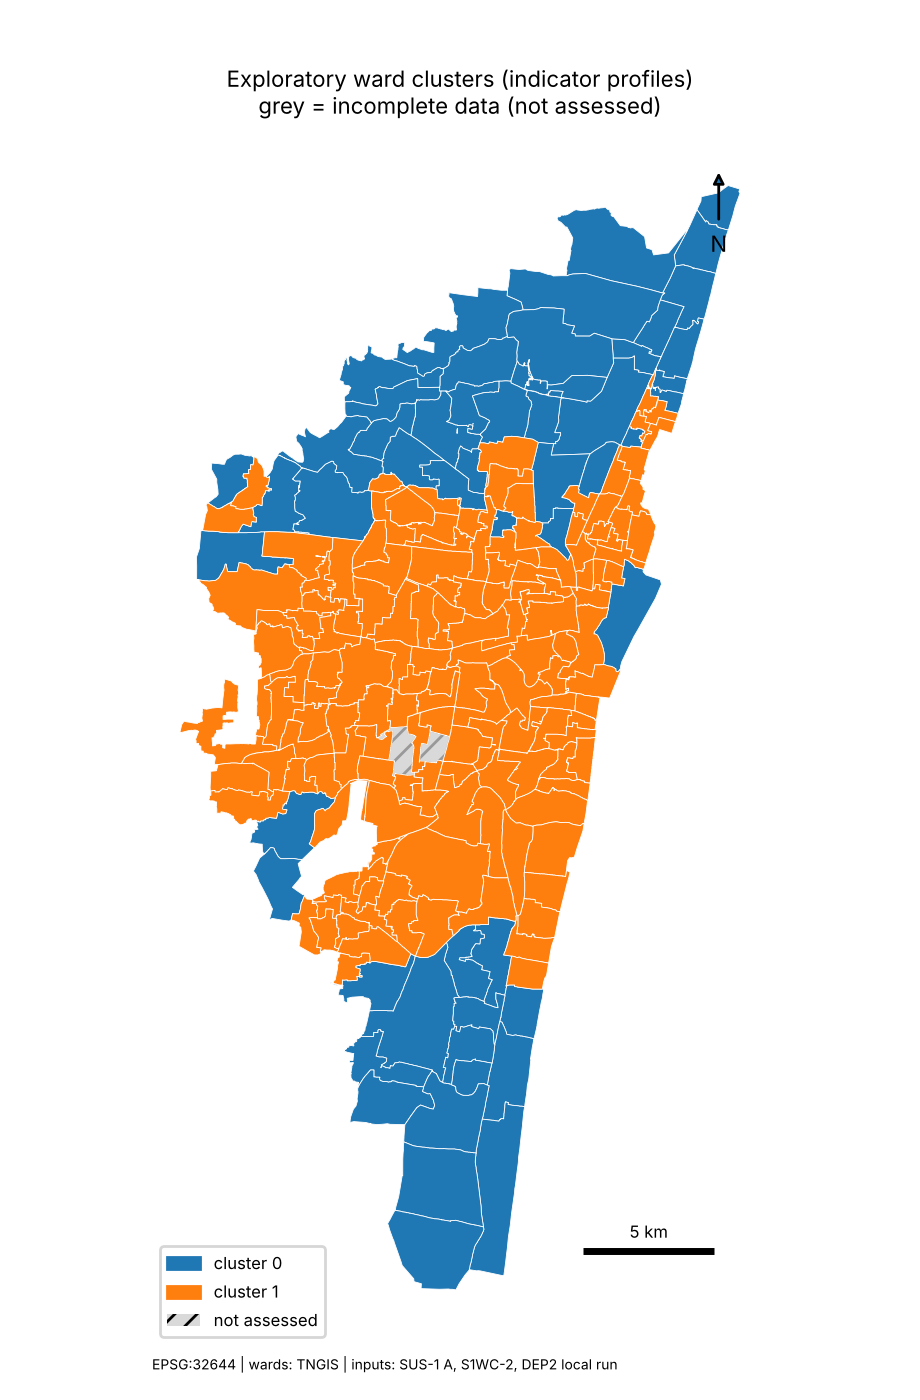
\includegraphics[width=0.62\columnwidth]{fig_cluster_map.png}
\caption{Two stable ward clusters in standardised indicator space. Grey wards lack complete data and are not assessed.}
\label{fig:clusters}
\end{figure}

\subsection{Presence-background analysis}
Prevalence is high: 119 of 198 wards are presences in 2015 and 147 of 198 in 2021. Under zone-blocked, buffered validation, no indicator set (physical; all indicators; all plus area) with either learner ranks presences above background beyond its permutation null (Fig.~\ref{fig:pb}). PB-AUC ranges from 0.39 to 0.54, with $p_{\mathrm{perm}}$ from 0.24 to 0.95. The only nominally significant result is the 2021 \emph{area-only} control (0.56, $p=0.04$). Pooled out-of-fold AUCs below 0.5 reflect prevalence differences between zones. The permutation nulls show the same shift (means 0.43--0.50), which is why every value is compared with its own null. In cross-event transfer the area control again does best (2015$\to$2021: 0.63). Indicator models score 0.56--0.60. Report intensity correlates weakly with all indicators ($|\rho|\le0.23$). The SUS-1 mean percentile is unrelated to 2021 intensity ($\rho=0.00$).

\begin{figure}[t]
\centering
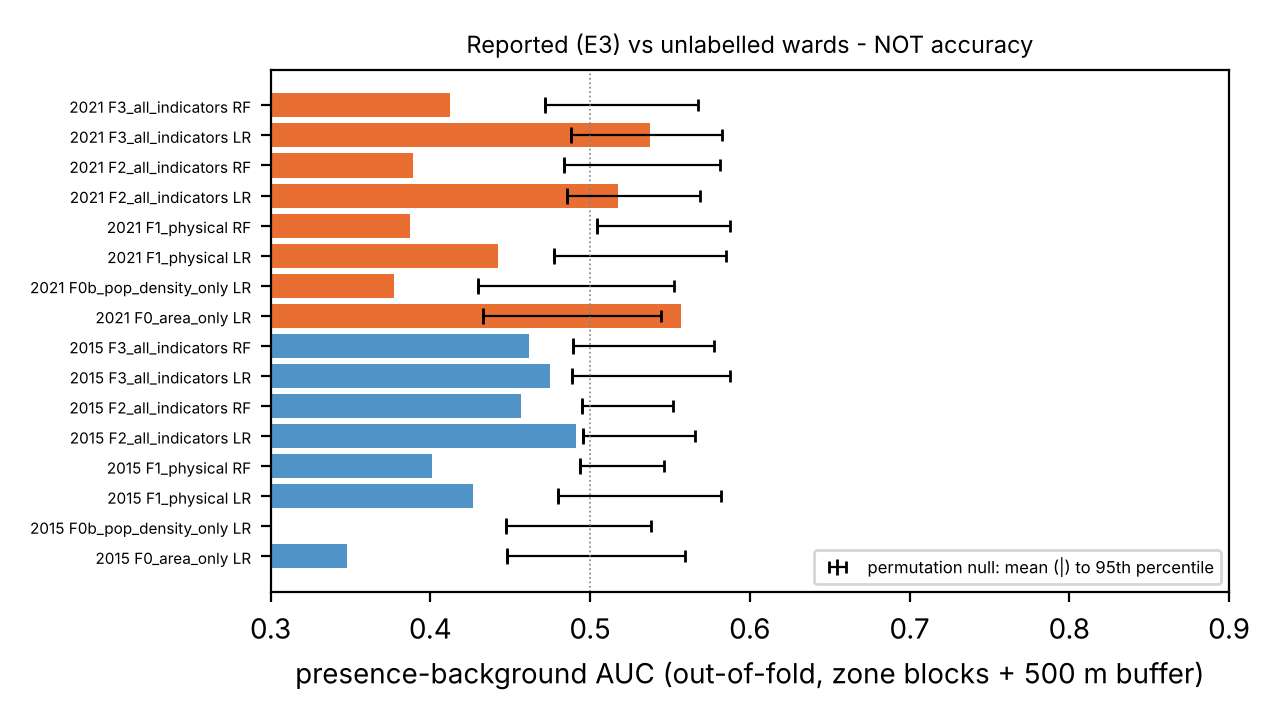
\includegraphics[width=\columnwidth]{fig_presence_background_auc.png}
\caption{Out-of-fold presence-background AUC (bars) and permutation nulls (mean to 95th percentile). This is a discrimination test of reported versus unlabelled wards, not an accuracy measure.}
\label{fig:pb}
\end{figure}

\section{Discussion}
The administrative lists are genuine evidence that flooding was reported in a ward. As training labels, however, they are dominated by reporting opportunity: larger wards contain more streets that can be listed. They also have year-level timing and no negatives. Fitting a classifier to them would reproduce reporting patterns and could yield high random-split scores that collapse under spatial blocking \cite{roberts2017cv}.

The radar result points in the same direction. Bright-VV diagnostics carry no detectable association with reported locations, consistent with the difficulty of urban SAR flood detection without coherence or building-aware methods \cite{mason2018urban,chini2019coherence}.

The structural finding has practical value regardless. In Chennai, terrain susceptibility peaks in peripheral, lower-density wards. Exposure and partial vulnerability peak in the core. Any combined index therefore depends strongly on weighting. We report the dimensions separately and flag five wards that are high on reported density, exposure and vulnerability only as an exploratory profile.

\emph{Limitations.}
\begin{itemize}
\item The study area is provisional.
\item GLO-30 is a surface model, and HAND is a Euclidean proxy.
\item The two population sources differ by a factor of about 3.
\item Social-sensitivity indicators are missing, and the partial vulnerability composite is sensitive to indicator choice (leave-one-out $\rho$ 0.56--0.85).
\item No E1 extent exists for any radar date.
\end{itemize}
The permutation nulls ignore spatial autocorrelation and are therefore, if anything, lenient.

\section{Conclusion}
With the flood evidence that can presently be verified for Chennai, a multi-source framework can describe susceptibility, exposure, partial vulnerability and the consistency of independent reports. It cannot learn or validate a flood predictor. Supervised modelling becomes defensible only with at least one of:
\begin{itemize}
\item mapped extents within a few days of a radar pass;
\item dated reports;
\item credible negatives;
\item an independent second event for testing.
\end{itemize}
The released pipeline, dashboard and data contract make this boundary explicit and testable.

\section*{Data and Code Availability}
Code, configuration, hash manifests and the exploratory outputs are in the project repository. Third-party documents whose licences are not stated are referenced by URL and SHA-256 rather than redistributed.

\bibliographystyle{IEEEtran}
\bibliography{references}

\end{document}
